\documentclass[a4paper, 12pt]{article}
\usepackage[a4paper, left=0.4cm, right=0.4cm, top=0.4cm, bottom=0.4cm, landscape]{geometry}
\usepackage{multicol}
\usepackage{listings}
\usepackage{enumitem}
\usepackage{graphicx}
\usepackage{courier}
\usepackage{vwcol}

\setitemize{noitemsep,topsep=0pt,parsep=0pt,partopsep=0pt,leftmargin=*}
\setenumerate{noitemsep,topsep=0pt,parsep=0pt,partopsep=0pt,leftmargin=*}
\lstset{
	belowskip=0.1em,
	aboveskip=0.1em,
    basicstyle=\ttfamily,
}

\begin{document}
\setlength\parindent{0pt}
\setlength{\multicolsep}{1.0pt plus 2.0pt minus 1.5pt}% 50% of original values
\scriptsize
\pagenumbering{gobble}

\begin{center}
{\normalsize\textbf{CS2106 Cheatsheet 19/20 S1 Midterms}}
\end{center}
\begin{multicols*}{3}
\noindent
{\small\textbf{Memory}}
\begin{itemize}
	\item Data: global variables
	\item Text: raw source code/instructions
	\item Stack: return address of caller/arguments/parameters/local variables
	\item Heap: dynamically allocated with \texttt{malloc}
\end{itemize}

\medskip

{\small\textbf{Process Abstraction}} \\
\textbf{Fork}
\begin{itemize}
	\item child $\rightarrow$ \texttt{fork() == 0}; parent $\rightarrow$ \texttt{fork() > 0}
	\item Data is copied; local changes made to child not reflected on parent
\end{itemize}
\begin{itemize}
	\item \texttt{exit(status)} causes normal process termination and the value of \texttt{status} is returned to the parent's call to \texttt{wait(\&status)}
	\begin{itemize}
		\item \texttt{status}: 8 LSB is exit status, next 8 is PID (\texttt{pid = status>>8})
	\end{itemize}
\end{itemize}
\textbf{Zombie Process}
\begin{itemize}
	\item Process that has completed execution (via \texttt{exit} system call) but still has an entry in the process table
	\item This occurs for child processes to allow the parent process to read its child’s exit status
	\item \texttt{kill} command has no effect on a zombie process
\end{itemize}
\textbf{Orphan Process}
\begin{itemize}
	\item Child process that is still executing, but whose parent has died
	\item When orphan processes die, they do not remain as zombie processes; they are waited on by init (PID 1)
\end{itemize}

\medskip

{\small\textbf{Process Scheduling}} \\
\textbf{Policies}
\begin{itemize}
	\item Non-preemptive/Cooperative: Process B will wait for process A to finish (or be blocked) before B starts running
	\item Preemptive: Every process given fixed time quota to run, and after time quota, process is suspended
\end{itemize}
\textbf{Definitions}
\begin{itemize}
	\item Timer Interrupt: OS scheduler will trigger every 1-10ms
	\item Time Quantum: A multiple of the timer interrupt
	\item Burst Time: time spent actually using CPU
	\item Turnaround Time: end time - enqueue time
	\item Response Time: start time - enqueue time
	\item Waiting Time: turnaround time - burst time
	\item Throughput: \# tasks finished per unit time
\end{itemize}
\textbf{First Come First Served (FCFS)}
\begin{itemize}
	\item Basically a FIFO queue; any process will eventually run
	\item Blocked process gets removed and added back to queue when ready
	\item Convoy Effect: many short processes waiting for a long process
\end{itemize}
\textbf{Shortest Job First (SJF)}
\begin{itemize}
	\item Select task with smallest \textbf{total} CPU time
	\item OS will need to know total CPU time for a task in advance
\end{itemize}
\textbf{Shortest Remaining Time First (SRT)}
\begin{itemize}
	\item Select task with smallest \textbf{remaining} CPU time
	\item Will preemptively stop another process to allow the shorter remaining time task to run (if such a task joins the queue)
\end{itemize}
\textbf{Round Robin (RR)}
\begin{itemize}
	\item Preemptive version of FCFS
	\item Each process given a pre-defined time quantum
	\item After time is up, process gets put back in queue if not yet finished
\end{itemize}
\textbf{Priority Scheduling}
\begin{itemize}
	\item Assign a priority to all tasks and do task with highest priority first
	\item Low priority tasks may be starved
	\item Hard to guarantee exact amount of CPU time given to each process
	\item May lead to priority inversion
	\begin{itemize}
		\item $P(H) > P(M) > P(L)$
		\item $L$ and $H$ shares CS but neither of them share CS with $M$
		\item $L$ is running in CS. $H$ also needs to run in CS. $H$ waits for $L$ to come out of CS. $M$ able to interrupt $L$ and starts running. $M$ runs till completion. $L$ resumes and starts running till the end of CS. $H$ finally enters CS and starts running.
	\end{itemize}
\end{itemize}
\textbf{Multi-Level Feedback Queue (MLFQ)}
\begin{itemize}
	\item If $P(A) > P(B)$, then $A$ runs
	\item If $P(A) = P(B)$, then $A$ and $B$ runs in RR
\end{itemize}
Settings:
\begin{itemize}
	\item New tasks will have highest priority
	\item If time quantum is used before finishing task, priority drops
	\item If task blocks before time slice is used, priority retains
\end{itemize}

\medskip

{\small\textbf{Inter Process Communication (IPC)}} \\
\textbf{Shared Memory}
\begin{lstlisting}[language=C]
void *shmat(int shmid, void *shmaddr, int shmflg);
\end{lstlisting}
\begin{itemize}
	\item Attaches the System V shared memory segment identified by \texttt{shmid} to the address space of the calling process. The attaching address is specified by \texttt{shmaddr} (if \texttt{NULL}, system chooses a suitable address)
	\item Region is identified/referred to by the user defined \texttt{int shmid} field, and not by the shared region address \texttt{shmaddr}
	\item Efficient: only the initial steps (create/attach) involves OS
	\item Ease of use: shared memory behaves as per normal memory space
	\item Hard to synchronise (see Race Condition)
\end{itemize}
\textbf{Message Passing}
\begin{itemize}
	\item Message to be passed is stored in kernel memory space
	\item Easy to synchronise when synchronous primitives are used
	\item Inefficient: every send/receive operation involves OS
\end{itemize}
\textbf{UNIX Pipe}
\begin{itemize}
	\item \texttt{A | B} means pipe output of \texttt{A} to input of \texttt{B}
	\item Data must be accessed in order (FIFO)
	\item Implicit synchronisation (wait when buffer is empty/full)
	\item read end: \texttt{0}, write end: \texttt{1}
\end{itemize}
\textbf{Signal}
\begin{lstlisting}[language=C]
sighandler_t signal(int signum, sighandler_t handler);
\end{lstlisting}
\begin{itemize}
	\item \texttt{signal()} sets the disposition of the signal \texttt{signum} to \texttt{handler}, which is either \texttt{SIG\_IGN}, \texttt{SIG\_DFL}, or the address of a defined function
\end{itemize}

\medskip

{\small\textbf{Threads}}
\begin{lstlisting}[language=C]
int pthread_create(pthread_t *tid, const pthread_attr_t 
    *attr, void *(*start_routine) (void *), void *arg);
\end{lstlisting}
\begin{itemize}
    \item Returns \texttt{0} on success, \texttt{!0} on errors
\end{itemize}
\begin{lstlisting}[language=C]
int pthread_exit(void *retval);
\end{lstlisting}
\begin{itemize}
    \item Terminates thread and sets \texttt{retval} to user defined value 
\end{itemize}
\begin{lstlisting}[language=C]
int pthread_join(pthread_t tid, void **retval)
\end{lstlisting}
\begin{itemize}
    \item Waits for \texttt{tid} and sets \texttt{retval} to \texttt{tid}'s return value
\end{itemize}
Threads in the same process shares
\begin{itemize}
	\item Memory Context: Variables, Text, Data, Heap
	\item OS Context: PID, files, etc
\end{itemize}
Pros:
\begin{itemize}
	\item Economy: multiple threads in same process requires less resources
	\item Resource Sharing: no need for IPC to pass messages around
	\item Responsiveness
	\item Scalability: take advantage of multiple CPUs
\end{itemize}
Cons:
\begin{itemize}
	\item Synchronisation of parallel execution of multiple threads
\end{itemize}
A single thread exits when:
\begin{itemize}
	\item Calling \texttt{pthread\_exit} or \texttt{pthread\_cancel}
	\item Returning from \texttt{start\_routine} (like \texttt{pthread\_exit} with \texttt{retval})
\end{itemize}
ALL threads exit when:
\begin{itemize}
	\item Any thread calls \texttt{exit()} or main thread returns from \texttt{main()}
\end{itemize}

\medskip

{\small\textbf{Synchronisation}} \\
\textbf{Race Condition} \\
Incorrect execution due to the unsynchronized access to a shared modifiable resource (global variable)
\begin{lstlisting}[language=C]
int globalVar = 0; //shared among all threads 
void* doSum(void* arg)
    int i, localVar = 0;
    for (i = 0; i < 50000; i++)
        localVar++;     
    globalVar += localVar;
\end{lstlisting}
Can be translated to
\begin{lstlisting}
lw  $r1, globalVar
add $r1, $r1, 50000 
sw  $r1, globalVar
\end{lstlisting}
Only 2 possible outcomes, \texttt{globalVar = 50000 || 100000}:
\begin{enumerate}
	\item Both threads do \texttt{lw} simultaneously (ie. both loads \texttt{0} to their \texttt{\$r1}) and both does their for loop and \texttt{sw 50000} to \texttt{globalVar}
	\item One thread finishes and \texttt{sw 50000}, the other thread then starts working, \texttt{lw 50000}, and finishes to \texttt{sw 100000} to \texttt{globalVar}
\end{enumerate}
\textbf{Critical Section (CS)} \\
Properties to maintain:
\begin{itemize}
	\item Mutual Exclusion: exactly one process at any point of time
	\item Progress: if no processs, one should enter
	\item Bounded Wait: there exists a bound, or limit, on the number of times other processes are allowed to enter their critical sections after a process has made request to enter its critical section and before that request is granted.
	\item Independence: process not executing in critical section should never block other process
\end{itemize}
Incorrect use can lead to: 
\begin{itemize}
    \item Deadlock: All processes blocked
    \item Livelock: Processes constantly change state to avoid deadlock
    \item Starvation: Some processes blocked forever
\end{itemize}
\textbf{Semaphore} \\
An object that consists of a counter, a waiting list (not necessarily FIFO) of processes, and two functions: \texttt{signal} and \texttt{wait}
\begin{itemize}
	\item \texttt{wait(S)}
	\begin{itemize}
		\item Decrement $counter$ by 1
		\item If $counter < 0$, add process to waiting list and block self
	\end{itemize}
	\item \texttt{signal(S)}
	\begin{itemize}
		\item Increment $counter$ by 1
		\item If $counter <= 0$, resume and remove a process from waiting list
	\end{itemize}
\end{itemize}
\begin{enumerate}
	\item If $counter < 0$, $|counter|$ is the number of waiting processes
	\item \texttt{wait()} may be blocked, but \texttt{signal()} is never blocked
	\item \texttt{wait()} and \texttt{signal()} must be \textbf{executed atomically}
	\item Deadlock is still possible with incorrect use of Semaphore
\end{enumerate}

\setlength{\columnsep}{-2cm}
\begin{multicols}{2}
\noindent
\begin{lstlisting}[language=C]
semaphore S = 3;
while (1)
    S.wait();
    // CS
    S.signal();
\end{lstlisting}
\vfill\null
\columnbreak
At most 3 processes can be in CS before CS is locked. Only when a process in CS finishes the work and calls \texttt{signal()} can another process enter CS.
\end{multicols}

\newpage

\textbf{Stack Frame Setup/Teardown}
\begin{itemize}
    \item An executable (binary) consists of Text and Data
    \item When under execution, memory context (text and data) and hardware context (general purpose registers, program counter) has to be known
\end{itemize}
On executing function call:
\begin{itemize}
    \item Caller: Pass arguments with registers and/or Stack
    \item Caller: Save return PC on Stack
    \item Transfer control from caller to callee
    \item Callee: Save registers used by callee; Save old FP, SP
    \item Callee: Allocate space for local variables of callee on stack
    \item Callee: Adjust SP to point to new stack top
\end{itemize}
On returning from function call:
\begin{itemize}
    \item Callee: Restore saved registers, FP, SP
    \item Transfer control from callee to caller using saved Process
    \item Caller: Continues execution in caller
\end{itemize}

\medskip
    
\textbf{Process Table}
\begin{center}
    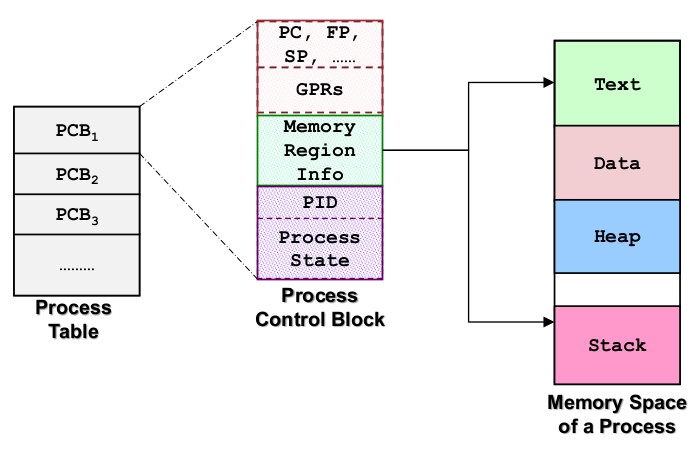
\includegraphics[scale=0.28]{process-table.png} \\
\end{center}

\textbf{System Calls}
\begin{center}
    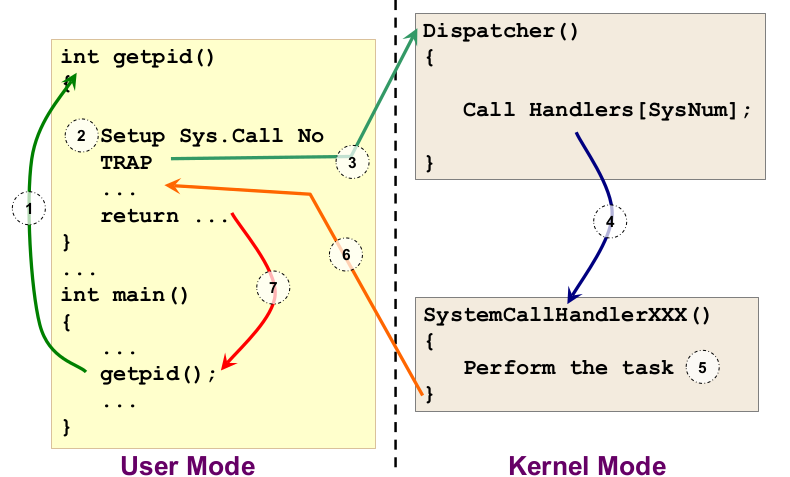
\includegraphics[scale=0.25]{system-call-mechanism.png}
\end{center}
\begin{enumerate}
    \item[(3)] Library call executes \texttt{TRAP} to switch from user mode to kernel mode
    \begin{itemize}
        \item Introduces overheads. Possibly require context switch
    \end{itemize} 
\end{enumerate}

\medskip

\textbf{State Processes}
\begin{center}
    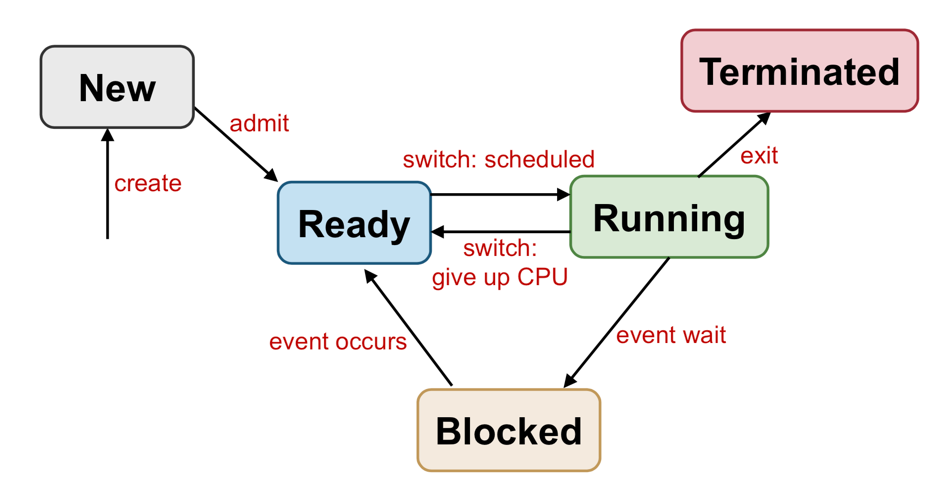
\includegraphics[scale=0.42]{5stateprocessmodel.png}
\end{center}
\begin{lstlisting}[language=C]
// before main starts: New -> Ready -> Running
int main() {
    int input, result;
    
    // Assuming I/O blocks
    // Running -> Blocked -> Ready -> Running
    printf("Give input below:\n");
    
    // Running -> Blocked -> 
    // [user input] -> Ready -> Running
    scanf("%d", &input);
    
    // assuming it takes a long time
    // Running -> Blocked -> Ready -> Running -> ...
    result = ComplexFunc( input );
    
    // write result to disk (takes long time)
    // Running -> Blocked -> Ready -> Running -> ...
    saveToDisk( result );
    
    return 0;
} // after main ends: Running -> Terminated
\end{lstlisting}

\medskip

\textbf{Multithread vs Multiprocess}
\begin{enumerate}
    \item Memory
    \begin{itemize}
        \item Threads share same memory space
        \item Processes each have independent memory space
        \item Multiprocess is used if memory usage is heavy
        \item Multiprocess is expensive if tasks share large amount of data
    \end{itemize}
    \item Overhead
    \begin{itemize}
        \item Thread creation is cheaper than forking
    \end{itemize}
    \item Protection
    \begin{itemize}
        \item Since processes have independent memory space, child processes can potentially hang, deface memory, without much negative behaviours to other processes
    \end{itemize}
    \item Hardware
    \begin{itemize}
        \item Whether hardware is capable of exploiting multiple threads
    \end{itemize}
    \item OS
    \begin{itemize}
        \item Some OSes favour one over the other
    \end{itemize}
\end{enumerate}

\medskip

\textbf{Peterson's Algorithm}
\begin{center}
    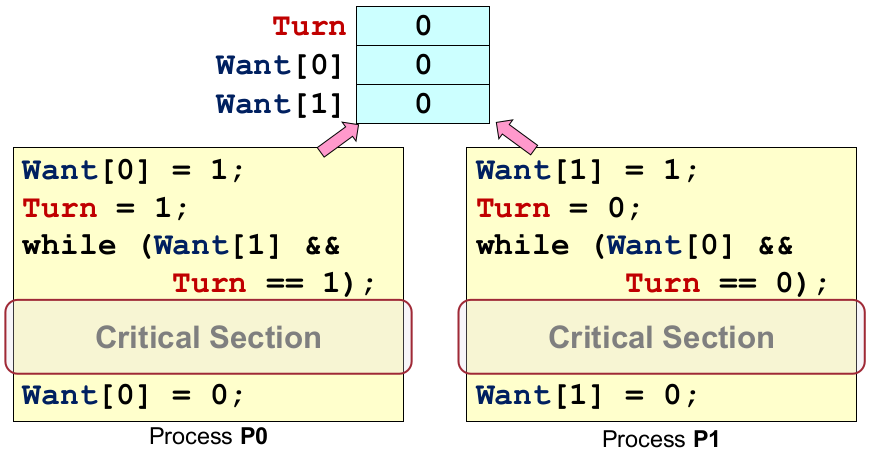
\includegraphics[scale=0.23]{petersons-algorithm.png}
\end{center}
\begin{itemize}
    \item Assumes writing to \texttt{Turn} is an atomic operation
    \item Busy Waiting: OS have to wait for time quantum of busy waiting task to finish to reschedule the other task $\rightarrow$ less efficient than sleep/block
\end{itemize}

\medskip 

\textbf{TestAndSet}
\begin{itemize}
    \item Write \texttt{1} to a memory location and return old value (atomic operation)
    \item Similar to a binary semaphore to maintain Mutual Exclusion
\end{itemize}
\begin{lstlisting}[language=C]
volatile int lock = 0;
void Critical()
    while (TestAndSet(&lock) == 1); // busy wait
    critical section // only one process can enter
    lock = 0 // release lock when finished with the CS
\end{lstlisting}

\medskip

\textbf{Producer Consumer}
\begin{center}
    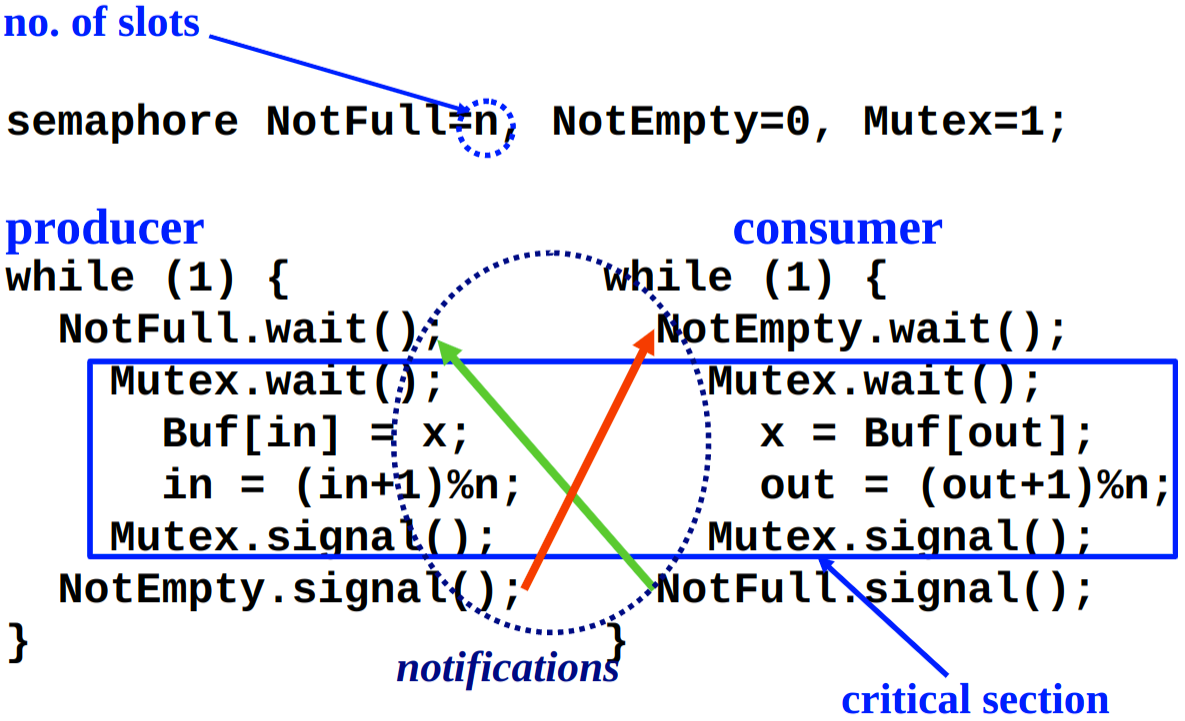
\includegraphics[scale=0.18]{producer-consumer.png}    
\end{center}

\medskip

\textbf{Dining Philosophers}
\begin{center}
    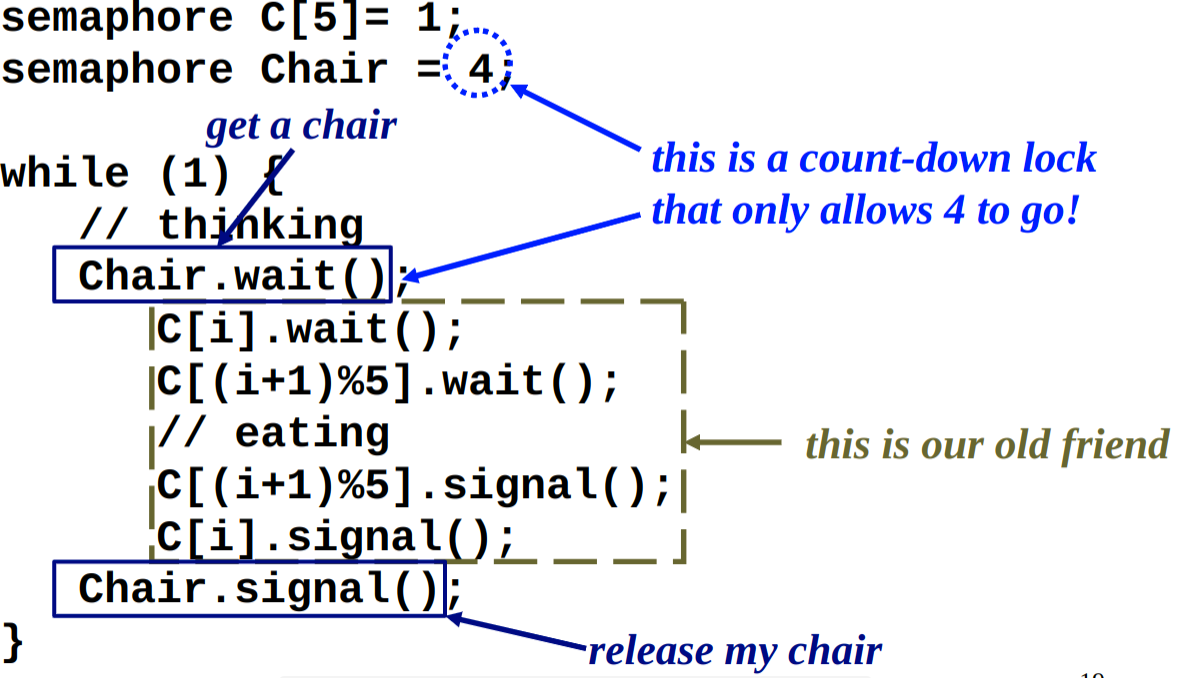
\includegraphics[scale=0.19]{philosophers-countdown.png}
\end{center}

\medskip

\textbf{Readers Writers}
\begin{center}
    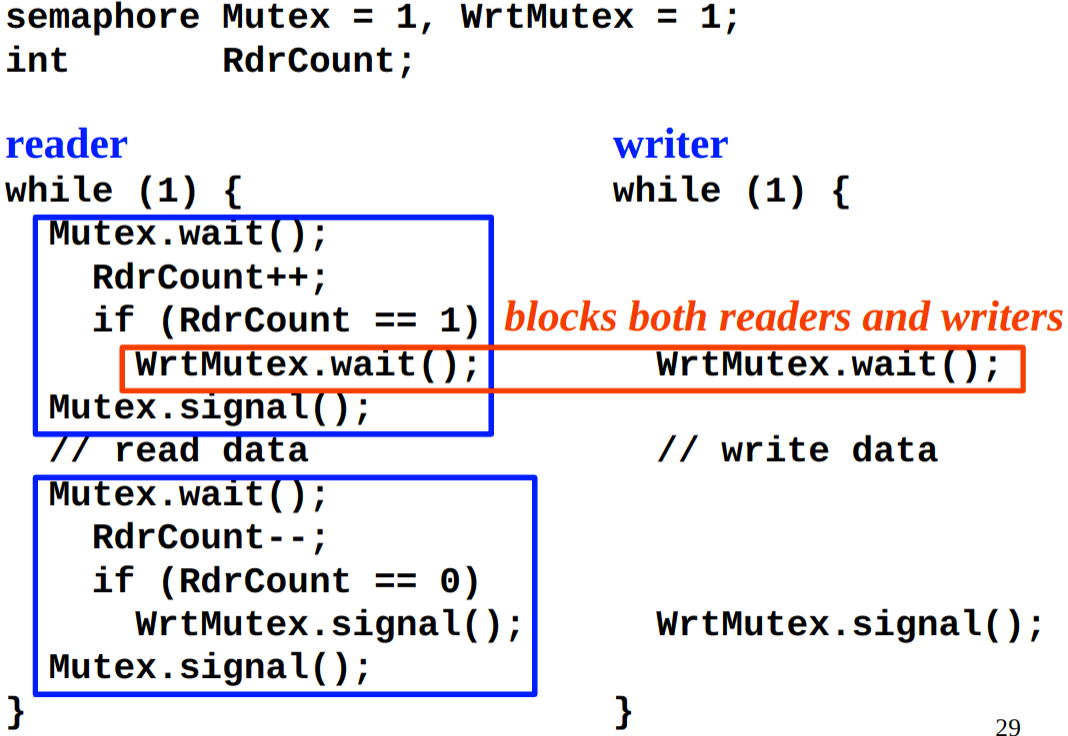
\includegraphics[scale=0.19]{readers-writers.png}
\end{center}

\end{multicols*}
\end{document}
